\documentclass{standalone}
\usepackage{pgfplots}
\pgfplotsset{compat=1.18}

\usetikzlibrary{decorations.markings}
\usetikzlibrary{arrows.meta}


\begin{document}

% Electromagnetic wave - circular polarization - color
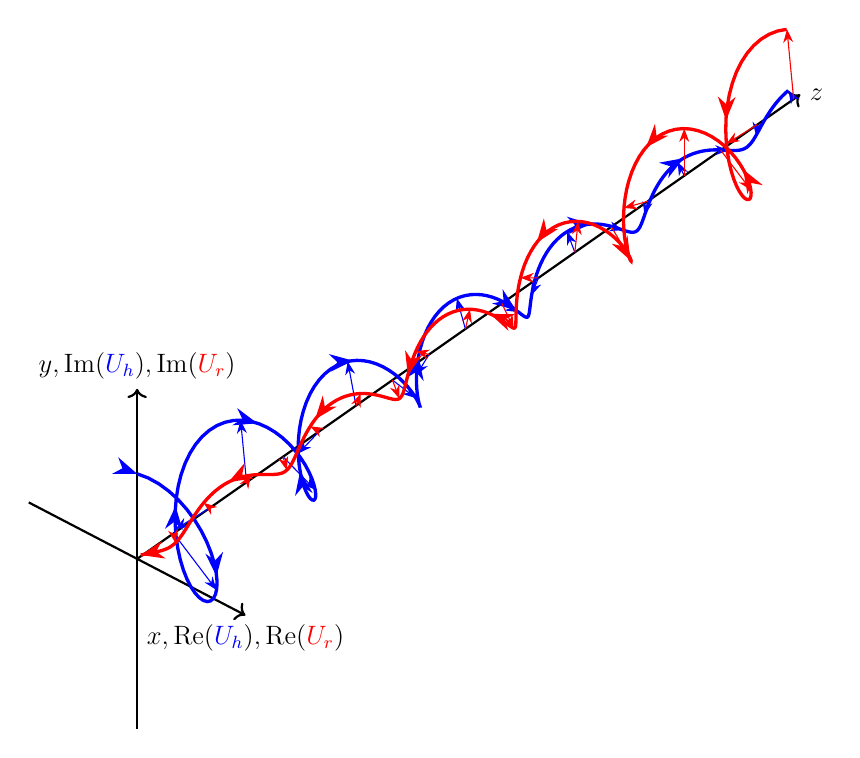
\begin{tikzpicture}[x=(35:0.9), y=(90:0.9), z=(-45:1.1),
axis/.style={black, thick,->},
vector/.style={>=Stealth,->},
scale=0.8, transform shape]

\large
\def\A{1.5}
\def\om{1.3}
\def\maxDomain{1.5}
\def\nNodes{6} % use even number
\def\nVectorsPerNode{2}
\def\N{\nNodes*40}
\def\xmax{\nNodes*pi/2*1.01}
\def\decay{0.15}
\pgfmathsetmacro\nVectors{\nVectorsPerNode*\nNodes*1.5}

% MAIN AXES
\draw[axis] (0,0,0) -- ++(\xmax*1.5,0,0) node[right] {$z$};
\draw[axis] (0,-\A*2.0,0) -- (0,\A*2.0,0) node[above] {$y, \mathrm{Im}({\color{blue}U_{h}}),
\mathrm{Im}({\color{red}U_{r}})$};
\draw[axis] (0,0,-\A*2.0) -- (0,0,\A*2.0) node[below] {$x, \mathrm{Re}({\color{blue}U_{h}}),
\mathrm{Re}({\color{red}U_{r}})$};

% waves
\draw[very thick,variable=\t,domain=0:\nNodes*pi/2*\maxDomain,samples=\N,blue, postaction={decorate},
decoration={markings, mark=between positions 0 and 1 step 0.1 with {\arrow{Stealth}}}]
plot (\t,{\A*exp(-\t*\decay)*cos(\om*2.0*deg(\t))},{\A*exp(-\t*\decay)*sin(\om*2.0*deg(\t))});

% draw vectors
\foreach \k [evaluate={\t=\k*pi/2/\nVectorsPerNode; \angle=\k*90/\nVectorsPerNode;}] in {1,...,\nVectors}{
    \draw[vector,blue] (\t,0,0) -- ++(0,{\A*exp(-\t*\decay)*cos(\om*2*\angle)},{\A*exp(-\t*\decay)*sin(\om*2*\angle)});
}

\draw[very thick,variable=\t,domain=0:\nNodes*pi/2*\maxDomain,samples=\N,red, postaction={decorate},
decoration={markings, mark=between positions 0 and 1 step 0.1 with {\arrowreversed{Stealth}}}]
plot (\t,{\A*exp(-(pi*5-\t)*\decay)*cos(\om*2.0*deg(\t)+180/4)},{\A*exp(-(pi*5-\t)*\decay)*sin(\om*2.0*deg(\t)+180/4)});


% draw vectors
\foreach \k [evaluate={\t=\k*pi/2/\nVectorsPerNode; \angle=\k*90/\nVectorsPerNode;}] in {1,...,\nVectors}{
    \draw[vector,red] (\t,0,0) --
    ++(0,{\A*exp(-(pi*5-\t)*\decay)*cos(\om*2.0*deg(\t)+180/4)},{\A*exp(-(pi*5-\t)*\decay)*sin(\om*2.0*deg(\t)+180/4)});
}

\end{tikzpicture}


\end{document}
